\documentclass[12pt]{article} 
\usepackage[left=2.5cm, right=2cm, top=2cm, bottom=2cm]{geometry} 
\usepackage{graphicx}
\usepackage[pages=some]{background}
\usepackage{titling}
\usepackage{tabularx}
\usepackage{tikz}
\usepackage{subfigure}
\usepackage{textcase}
\usepackage{newtxtext}
\usepackage{enumitem}
\usepackage{fancyhdr}
\usepackage{graphicx}

\pagestyle{fancy}
\fancyhf{} 
\renewcommand{\headrulewidth}{0pt} 
\rhead{\#1810009}

\begin{document}
\section*{(B) Answers to the Questions:}
\begin{enumerate}[label=(\roman*)]
    \item \textbf{No. of cylinder rings, their types and functions:} \\
    There are generally two types of cylinder rings, a) Oil ring, b) Compression ring. Cylinder rings are also known as piston rings. Their types and functions are as follows:
    
    a) Oil Rings:
    \begin{itemize}
      \item There is one oil control ring per piston. Oil control rings consist of two parts: the scraper ring and the expander ring. Oil control rings help regulate the distribution of oil along the cylinder wall. They prevent excessive oil from entering the combustion chamber while ensuring adequate lubrication of the cylinder wall. The scraper ring scrapes excess oil off the cylinder wall, while the expander ring maintains tension and ensures proper contact.
    \end{itemize}
    
    b) Compression Rings:
    \begin{itemize}
      \item There are two or three compression rings per piston. The compression rings include the top compression ring and the second compression ring.
      Compression rings seal the combustion chamber during the compression and power strokes of the engine. They prevent the escape of high-pressure gases from the combustion chamber and ensure maximum compression, promoting efficient combustion.
    \end{itemize}
    
    \vspace*{0.3cm}
    
    \item \textbf{No. of bearings, their types and functions:} \\
    There are total 6 bearings, 4 ball bearings and 2 journal bearings. Two ball bearings are installed on both sides of the crankshaft and camshaft, and they are referred to as short end ball bearings. The other two ball bearings are placed between the connecting rod and camshaft, known as long end ball bearings. These four bearings assist in the rotation of the camshaft and crankshaft, enabling the transmission of power.

    The journal bearings are mounted on the two ends of the connecting rods, which connect the pistons and crankshafts. Therefore, they play a crucial role in the combustion process and power transmission. 

    \vspace*{0.3cm}
    \item \textbf{No. of valves and mention which one was bigger:} \\
    There are an intake valve and an exhaust valve. The intake valve allows air and fuel to enter the combustion chamber, while the exhaust valve lets out the combustion by-products. The intake valve is usually larger to accommodate a higher volume of air and fuel for efficient combustion.  A larger intake valve helps facilitate the smooth and unrestricted flow of the air-fuel mixture into the combustion chamber. The exhaust valve is smaller as it deals with expelling exhaust gases. The exhaust gases are under higher pressure compared to the intake mixture, so a smaller valve can effectively handle the flow of these gases during the exhaust stroke.

    \item \textbf{Location of Cooling water pump:} \\
    There was no cooling water pump in this engine. Water is cooled by natural convection. 

    \item \textbf{Fuel injection type NG of holes in each nozzle:} \\
    The fuel injector type was multi-point airless fuel injector. There are 4 holes in each nozzles. 
\end{enumerate}

\pagebreak
\section*{(C) Discussion:}
During the experiment on dismantling and assembling a (CI) diesel engine, we gained valuable insights into the internal components and functioning of a typical diesel engine. The process involved carefully disassembling the engine, inspecting each component, and then reassembling it to its original state. This hands-on activity provided us with a practical understanding of the various parts and their roles in the engine's operation.\\

One of the primary objectives of the experiment was to familiarize ourselves with the construction and arrangement of components within the diesel engine. We observed components such as the cylinder head, pistons, connecting rods, crankshaft, camshaft, valves, fuel injectors, and various bearings. By visually examining these parts, we gained a better understanding of their functions and how they work together to convert fuel into mechanical energy.\\

The process of dismantling the engine allowed us to observe any wear and tear, damage, or malfunctions in the components. We inspected the cylinder walls for signs of scoring or excessive wear, checked the pistons and piston rings for wear and proper fit, and examined the bearings for any signs of damage or inadequate lubrication. This analysis provided valuable insights into the maintenance requirements of a diesel engine and the importance of regular inspections and servicing.\\

Assembling the engine back together required careful attention to detail. We ensured that each component was properly aligned and securely fastened. Torque specifications were followed to prevent over-tightening or under-tightening of bolts and nuts. Throughout the experiment, safety precautions were strictly followed. We wore personal protective equipment, used appropriate tools, and exercised caution when handling delicate or heavy components. This emphasized the importance of safety protocols in a practical laboratory setting and reinforced the need for responsible and careful work practices.\\

In conclusion, the dismantling and assembling of a diesel engine provided us with a hands-on experience to understand the internal workings and construction of the engine. It enhanced our knowledge of the various components and their functions, as well as the importance of regular maintenance and proper assembly techniques. This experiment served as a valuable learning opportunity and contributed to our overall understanding of internal combustion engines.\\

\pagebreak

\begin{figure}
  \subfigure[Piston]{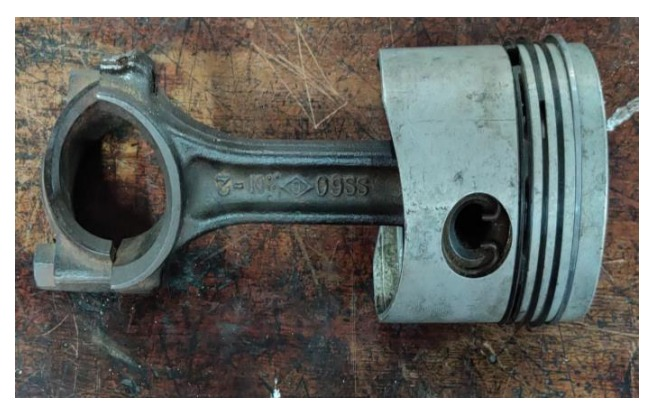
\includegraphics[width=0.32\linewidth]{img/piston.jpeg}}
  \hfill
  \subfigure[Engine Head]{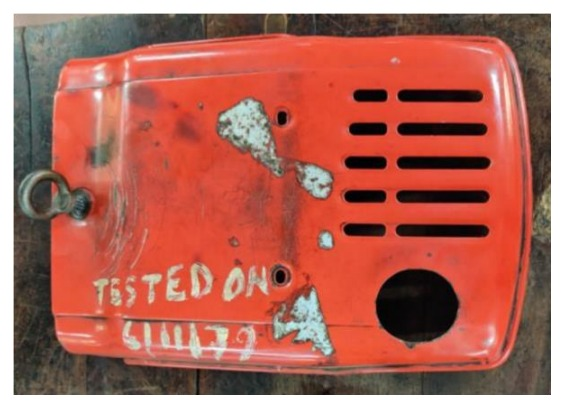
\includegraphics[width=0.32\linewidth]{img/engine_head.jpeg}}
  \hfill
  \subfigure[Cylinder Head]{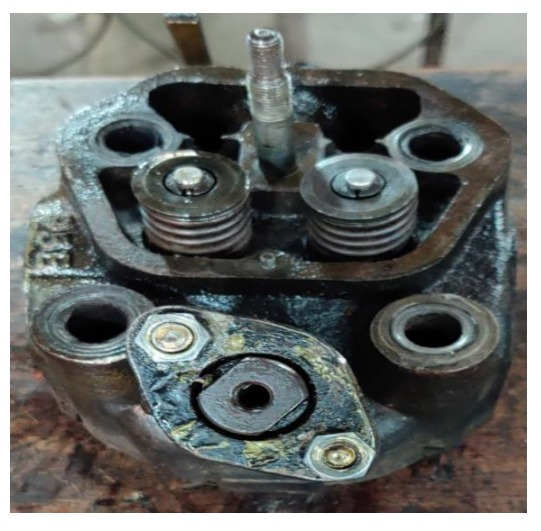
\includegraphics[width=0.32\linewidth]{img/cylinder_head.jpeg}}
  \vspace{0.2cm}

  \subfigure[Push Rod]{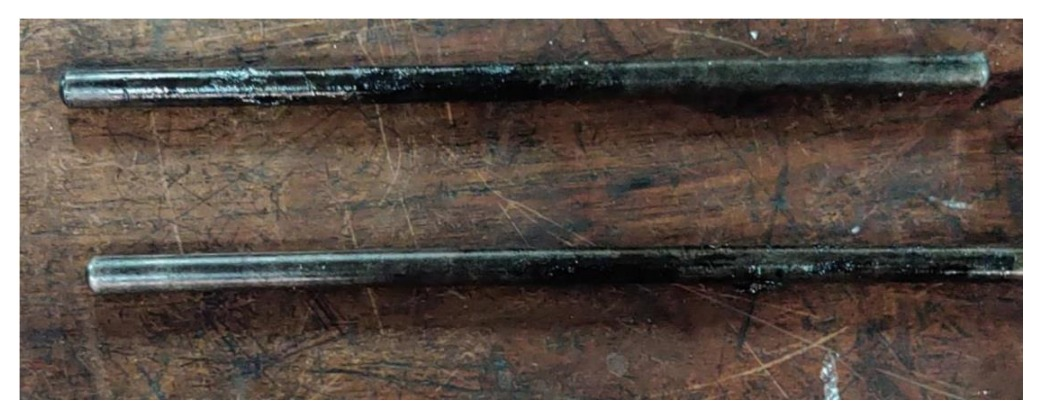
\includegraphics[width=0.32\linewidth]{img/push_rod.jpeg}}
  \hfill
  \subfigure[Exhaust Manifold]{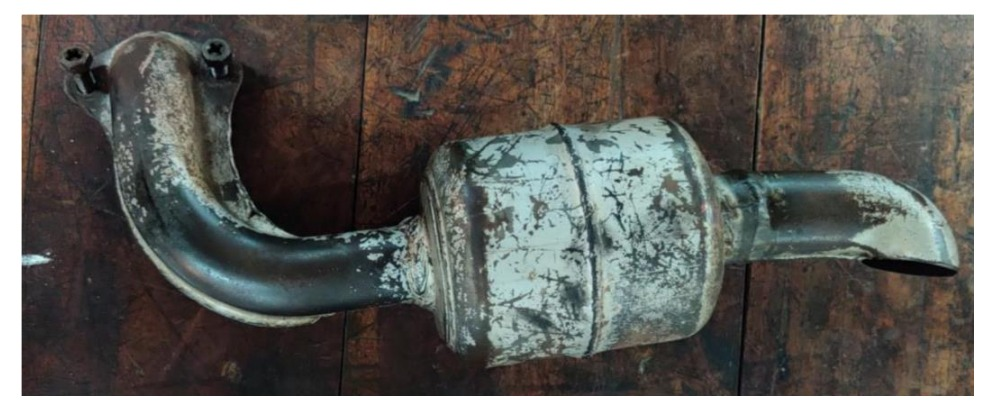
\includegraphics[width=0.32\linewidth]{img/exhaust_manifold.jpeg}}
  \hfill
  \subfigure[Rear End Cover]{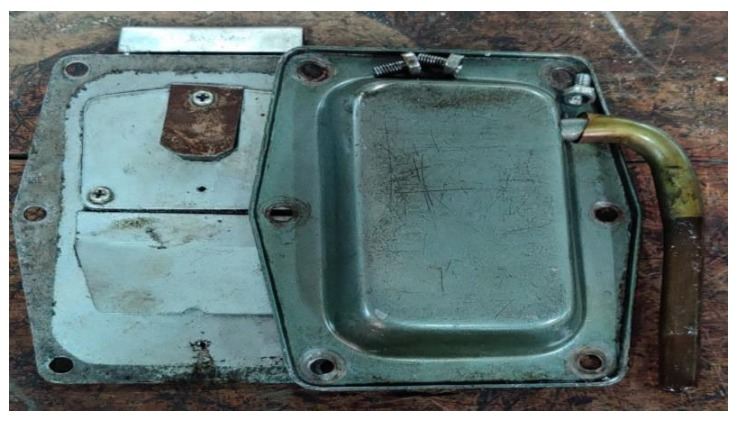
\includegraphics[width=0.32\linewidth]{img/rear_end.jpeg}}
  \vspace{0.2cm}

  \subfigure[Front Head Cover]{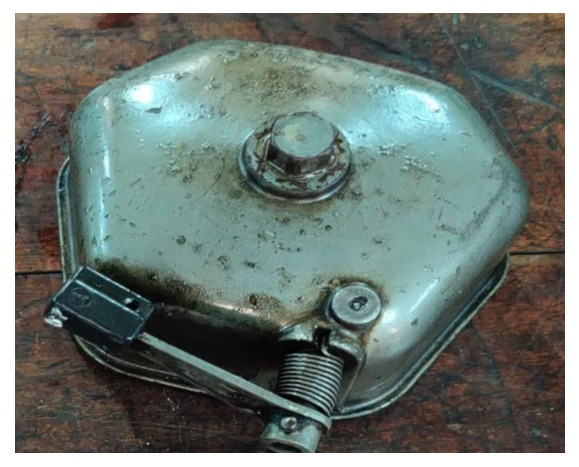
\includegraphics[width=0.32\linewidth]{img/front_head_cover.jpeg}}
  \hfill
  \subfigure[Rocker Arm]{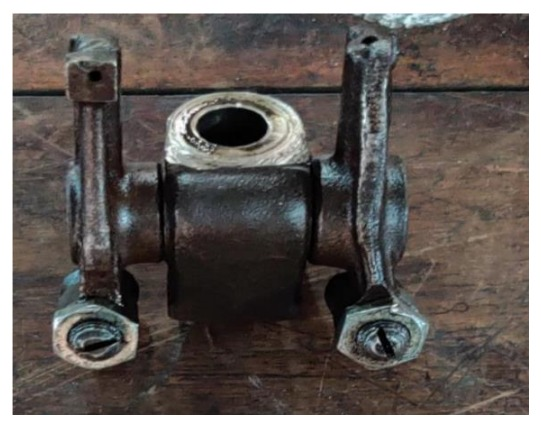
\includegraphics[width=0.32\linewidth]{img/arm_rocker.jpeg}}
  \hfill
  \subfigure[Timing Cover]{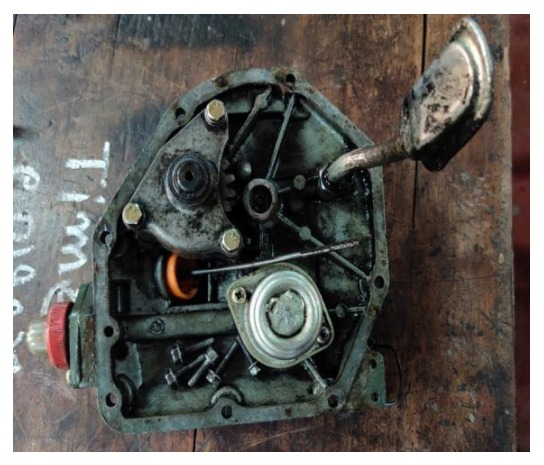
\includegraphics[width=0.32\linewidth]{img/timing_cover.jpeg}}
  \vspace{0.2cm}
  \vspace{0.2cm}

  \subfigure[Flywheel]{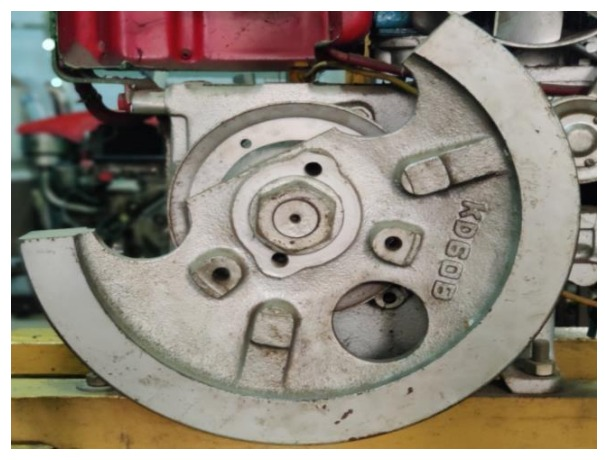
\includegraphics[width=0.32\linewidth]{img/flywheel.jpeg}}
  % \hfill
  \subfigure[Fuel Filter]{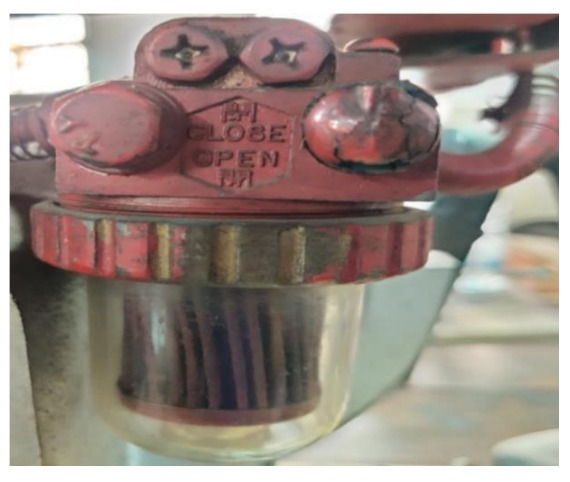
\includegraphics[width=0.32\linewidth]{img/fuel_filter.jpeg}}
  \caption{Components of Diesel Engine}
\end{figure}
  \pagebreak
  
(a) \textbf{Piston:} The piston is a cylindrical component that moves up and down within the cylinder bore. It is connected to the connecting rod and transfers the force generated by the combustion of fuel to the crankshaft.\\

(b) \textbf{Engine Head:} The engine head, also known as the cylinder head, is a critical component that seals the top of the engine block. It contains the combustion chamber, intake and exhaust ports, and houses various valves, spark plugs (in gasoline engines), or fuel injectors (in diesel engines).\\

(c) \textbf{Cylinder Head:} The cylinder head is the uppermost part of the engine block. It provides housing for the cylinders and plays a vital role in sealing the combustion chambers. It also contains passages for coolant circulation and often incorporates the engine head as well.\\

(d) \textbf{Push Rod:} A push rod is a long, slender rod that transmits the upward motion of the camshaft or lifter to actuate the rocker arm. \\

(e) \textbf{Exhaust Manifold:} The exhaust manifold is a component that collects the exhaust gases from each cylinder and directs them into the exhaust system. It is bolted to the cylinder head and typically made of cast iron or stainless steel to withstand high temperatures.\\

(f) \textbf{Rear End Cover:} The rear end cover, also known as the rear seal cover, is a protective housing located at the back of the engine. It covers the rear main seal, which prevents oil leaks where the crankshaft exits the engine block.\\

(g) \textbf{Front Head Cover:} The front head cover is a protective housing located at the front of the engine. It covers the front of the cylinder head and other components, providing protection and housing for various engine accessories like the timing gears or belts.\\

(h) \textbf{Rocker Arm:} The rocker arm is a pivoting lever that transfers the motion from the push rod to open and close the engine's valves. It acts as an intermediary between the push rod and the valve, providing the necessary mechanical advantage to operate the valve.\\

(i) \textbf{Timing Cover:} The timing cover is a protective housing that encloses the timing components of the engine. It covers the timing chain or timing belt, camshaft(s), and other associated components. It helps keep these components lubricated and protects them from contaminants.\\

(j) \textbf{Flywheel:} The flywheel is a large, heavy wheel mounted on the crankshaft. It stores rotational energy and helps maintain engine momentum, providing smooth operation and reducing vibrations.\\

(k) \textbf{Fuel Filter:} The fuel filter is a device that cleans the fuel before it reaches the engine. It removes contaminants such as dirt, rust, and other particles that could potentially damage the fuel injectors or carburetor. It ensures that only clean fuel enters the combustion chambers, promoting proper engine performance and longevity.\\


\end{document}
